\documentclass[conference]{IEEEtran}
\IEEEoverridecommandlockouts
\usepackage{cite}
\usepackage{amsmath,amssymb}
\usepackage{graphicx}
\usepackage{booktabs}
\usepackage{url}
\usepackage[hidelinks]{hyperref}
\graphicspath{{../figures/}}

\begin{document}

\title{Do Network Elements Have a Grammatical Fingerprint?\\
A Pre-Registered Test on Cellular Telemetry}

\author{\IEEEauthorblockN{Autonomous Research Agent (Claude, Anthropic)}
\IEEEauthorblockA{CNSM 2026 AI-Generated Paper Track\\
Human contribution: procedural decisions only (see Disclosure Statement)}}

\maketitle

\begin{abstract}
We test whether the symbolic grammar of a network element's telemetry
identifies the element, independent of traffic volume. Using the Telecom
Italia Milano cellular grid, we discretize per-cell internet-activity time
series with SAX and train a Markov-chain classifier and an LSTM on a strictly
temporal train/test split. Source identification greatly exceeds chance: at
$N{=}50$ elements a shallow order-2 Markov model attains $0.51$ accuracy on
held-out, same-regime data, $25.5\times$ the $0.02$ chance rate (permutation
$p<0.001$, Table~\ref{tab:byn}). The effect is largely temporal: on
amplitude-adjusted (AAFT) surrogates accuracy collapses to $0.139$
(Table~\ref{tab:controls}). However, a mean-traffic-level baseline reaches
$0.46$ at $N{=}50$ and $0.85$ at $N{=}10$ (Table~\ref{tab:controls}), so
volume is a second, at small $N$ stronger, fingerprint; the grammatical
fingerprint survives only because it is measured after per-element
normalization. The shallow model beats the LSTM ($0.21$), so a sequence model
adds nothing here (S1). The measured data-volume threshold is $N^\ast<12$
symbols, one-to-two orders of magnitude below the $1299$-symbol value predicted
by the authors' prior scaling proposal (Table~\ref{tab:h2}): the two are
\emph{inconsistent}. During the documented Christmas regime change, grammatical
drift is detected a median $54$\,h (95\% CI $18$--$90$\,h) before first-order
drift (Fig.~\ref{fig:drift}). Network telemetry does carry a stable,
volume-independent grammatical fingerprint that drifts early---but it coexists
with a simpler volume fingerprint, and its data threshold does not follow the
prior relation.
\end{abstract}

\begin{IEEEkeywords}
network telemetry, symbolic dynamics, device fingerprinting, SAX, drift
detection.
\end{IEEEkeywords}

\section{Introduction}
Discretized activity traces of complex systems can carry source-identifying
structure: the symbolic grammar of a trace may reveal \emph{which} source
produced it, independent of whether the trace is anomalous. Learning the
``noise fingerprint'' of quantum devices is one demonstration~\cite{martina2022noise}.
We ask whether the same holds for network telemetry: \emph{do network elements
have a grammatical fingerprint?} Concretely, does the sequence of symbols
obtained by discretizing a cell's telemetry identify that cell, and does the
identifying signal live in temporal (grammatical) structure rather than in the
traffic volume alone?

This question is pre-registered. Before any data was downloaded we fixed the
dataset, the element count, the SAX and model grid, the temporal split, the
controls, and---critically---the operational mapping used to compare against a
prior scaling proposal (Section~\ref{sec:method}). We report the obtained
results without post-hoc reframing: the central hypothesis is supported, one
secondary hypothesis is refuted, and an important confound (volume) is found to
be a competing fingerprint in its own right.

\section{Related Work}
\textbf{Traffic and device fingerprinting.} Website-fingerprinting attacks
recover the site behind an encrypted Tor connection from packet-timing and
direction features, reaching $>95\%$ accuracy with deep
networks~\cite{sirinam2018deep,rimmer2018automated}. These operate on
\emph{flow-level} features (packet sizes, directions, inter-arrival times) and
target \emph{content} (which page). We differ on both axes: our input is a
coarse, aggregated activity \emph{level} sampled every 10~minutes, and our
target is the \emph{infrastructure element} (which cell), not the traffic
content. What we add is the isolation of the \emph{grammatical} component:
by z-normalizing per element before symbolization, and by comparing against
surrogate and volume baselines, we separate ``which cell'' as told by symbol
\emph{order} from ``which cell'' as told by mean load.

\textbf{Symbolic dynamics.} SAX~\cite{lin2007sax} maps a z-normalized,
piecewise-aggregated series to a symbol string, enabling Markov and $n$-gram
models over telemetry. Surrogate-data testing~\cite{theiler1992surrogate}
provides the AAFT null that preserves the marginal amplitude distribution while
destroying temporal structure; we use it to decide whether identification is
grammatical or merely distributional.

\textbf{Substrate-independent thresholds.} The starting prompt cites the
authors' earlier proposal of a data-volume threshold
$N^\ast=H_0\,B\,C\,Q^{\alpha}$ with $\alpha\approx-0.77$, from quantum-circuit
and EEG traces. We could not locate a peer-reviewed publication of this
relation; we therefore treat it strictly as a pre-registered proposal (stated
in our public repository), not an established law, and test consistency
quantitatively (Section~\ref{sec:results}).

\section{Method}\label{sec:method}
\textbf{Data.} Telecom Italia Big Data Challenge, Milano
grid~\cite{barlacchi2015milano} (Harvard Dataverse
\texttt{doi:10.7910/DVN/EGZHFV}, v1.3, ODbL~1.0): per-cell activity on a
$100\times100$ grid, 10-minute resolution, 62 days (2013-11-01 to 2014-01-01).
Each cell is one network element; the internet channel is used. All 62 daily
files were MD5-verified against the repository metadata.

\textbf{Elements.} $N$ cells are chosen by stratified sampling across deciles
of training-period mean activity (seed 42), excluding cells with $>5\%$ missing
training intervals ($9{,}972$ eligible). Primary $N{=}50$; scaling uses
$N\in\{10,25,50,100\}$.

\textbf{Discretization and models.} Per-element z-normalization uses
\emph{training-period} statistics only (volume control), then PAA$+$SAX. The
shallow baseline is an order-$k$ Markov classifier assigning a window to the
element of maximum sequence log-likelihood; the sequence model is a
single-layer LSTM (hidden~64, embedding~16), with only its epoch count tuned by
early stopping inside the training period.

\textbf{Split.} Train 2013-11-01--12-12. The held-out period is split at a
fixed calendar boundary into two disjoint windows: \textbf{Test-A}
(12-13--12-20, same regime), which carries \emph{all} confirmatory statistics,
and \textbf{Test-B} (12-21--01-01), used \emph{only} for drift (H3). This keeps
H1 (stability) and H3 (drift) unconfounded. Hyperparameters were frozen by a
repository commit before the single test evaluation.

\textbf{Sweep (training only).} Rolling-origin validation over alphabet
$a\in\{4,6,8\}$, PAA window $w\in\{3,6,12\}$ samples, order $k\in\{1,2,3\}$,
selected at $L{=}48$ symbols (Table~\ref{tab:sweep}). Selection:
$a{=}8,\,w{=}12$ (120~min), $k{=}2$.

\textbf{Controls.} (i) Label-permutation test, $1000$ permutations. (ii) AAFT
surrogates generated from the \emph{raw} series, then discretized with the
frozen SAX parameters. (iii) Volume confound: per-element normalization plus a
mean-level-only baseline on the un-normalized series.

\textbf{H2 mapping (pre-registered).} $H_0$: order-0 symbol entropy (bits);
$B=\log_2 a$; $C=N$; $Q$: mean pairwise Jensen--Shannon divergence between
per-element order-1 transition distributions (bits); $\alpha=-0.77$, not
refitted. $N^\ast_{\text{meas}}$ is the interpolated sequence length at which
accuracy crosses the permutation band (bootstrap CI over elements). Consistency
holds iff $N^\ast_{\text{pred}}=H_0 B C Q^{-0.77}$ lies in that CI.

\textbf{H3.} Identical CUSUM (Page--Hinkley as robustness check) on symbolic
signals (per-element log-likelihood; sliding Jensen--Shannon divergence of the
transition distribution vs.\ the training reference) and on raw first-order
signals (sliding mean, variance), 24\,h windows at 6\,h stride, thresholds
calibrated identically on the training period. Lead time is the raw-signal
alarm time minus the symbolic alarm time, bootstrapped over elements. Global
seed 42; one command reproduces every result.

\section{Results}\label{sec:results}

\begin{table}[t]
\caption{Validation accuracy of the shallow model in the training-only sweep
(selection at $L{=}48$, $N{=}50$). Selected cell in bold.}
\label{tab:sweep}
\centering\small
\begin{tabular}{ccccc}
\toprule
$a$ & $w$ & $k{=}1$ & $k{=}2$ & $k{=}3$\\
\midrule
4 & 3 & 0.144 & 0.153 & 0.162\\
4 & 6 & 0.162 & 0.231 & 0.258\\
4 & 12 & 0.273 & 0.367 & 0.413\\
6 & 12 & 0.353 & 0.427 & 0.440\\
8 & 6 & 0.282 & 0.324 & 0.322\\
8 & 12 & 0.433 & \textbf{0.453} & 0.427\\
\bottomrule
\end{tabular}
\end{table}

\begin{table}[t]
\caption{H1: Test-A identification accuracy (order-2 Markov). Every cell has
permutation $p<0.001$. Chance $=1/N$.}
\label{tab:byn}
\centering\small
\begin{tabular}{lccccc}
\toprule
$N$ & chance & $L{=}12$ & $L{=}24$ & $L{=}48$ & $L{=}96$\\
\midrule
10 & 0.100 & 0.325 & 0.475 & 0.500 & 0.600\\
25 & 0.040 & 0.315 & 0.400 & 0.560 & 0.680\\
50 & 0.020 & 0.270 & 0.405 & 0.510 & 0.680\\
100 & 0.010 & 0.200 & 0.320 & 0.445 & 0.510\\
\bottomrule
\end{tabular}
\end{table}

\textbf{H1 (fingerprint): supported.} Identification greatly exceeds chance for
every $N$ and every sequence length, with permutation $p<0.001$ throughout
(Table~\ref{tab:byn}, Fig.~\ref{fig:accL}). At the primary operating point
($N{=}50$, $L{=}48$) accuracy is $0.51$ against a $0.02$ chance rate. Accuracy
grows with sequence length and degrades gracefully with $N$
(Fig.~\ref{fig:accN}). H0 is rejected.

\begin{table}[t]
\caption{Controls at $N{=}50$, $L{=}48$ (Test-A). All $p<0.001$.}
\label{tab:controls}
\centering\small
\begin{tabular}{lcc}
\toprule
Classifier / control & accuracy & chance\\
\midrule
Markov, order 2 (grammatical) & 0.510 & 0.020\\
LSTM (sequence model, S1) & 0.210 & 0.020\\
Mean-level baseline (raw volume) & 0.460 & 0.020\\
AAFT surrogate (Markov) & $0.139\pm0.034$ & 0.020\\
\bottomrule
\end{tabular}
\end{table}

\textbf{Grammar vs.\ marginal (surrogate control).} On AAFT surrogates the
Markov classifier falls from $0.51$ to $0.139\pm0.034$
(Table~\ref{tab:controls}). Most of the identifiability is therefore temporal
(grammatical), as claimed; but $0.139$ is still $7\times$ chance, so the
marginal symbol distribution alone carries a non-trivial share. The grammar
claim is thus supported but not exclusive.

\textbf{Volume confound.} The mean-level-only baseline, using nothing but each
window's raw average, reaches $0.46$ at $N{=}50$ and $0.85$, $0.60$, $0.195$ at
$N{=}10,25,100$. Volume is thus an independent fingerprint that at small $N$ is
\emph{stronger} than the grammatical one. Because the Markov classifier acts on
per-element z-normalized data, its $0.51$ is volume-independent: the two
fingerprints coexist. Honestly stated, ``grammatical fingerprint'' is one of at
least two identifying channels, not the sole explanation of identifiability.

\textbf{S1 (shallow vs.\ sequence): shallow suffices.} The LSTM reaches only
$0.21$ at $N{=}50$, $L{=}48$ (Table~\ref{tab:controls}), well below the Markov
model. A sequence model adds nothing here, consistent with modest per-element
data; we report this plainly rather than tuning the LSTM further.

\begin{table}[t]
\caption{H2: measured vs.\ predicted data-volume threshold $N^\ast$ (symbols).
Measured is left-censored at the shortest tested length ($L{=}12$).}
\label{tab:h2}
\centering\small
\begin{tabular}{lcccc}
\toprule
$N$ & $H_0$ (bits) & $Q$ (bits) & $N^\ast_{\text{pred}}$ & $N^\ast_{\text{meas}}$\\
\midrule
10 & 2.96 & 0.142 & 400 & $<12$\\
25 & 2.98 & 0.217 & 724 & $<12$\\
50 & 2.98 & 0.250 & 1299 & $<12$\\
100 & 2.98 & 0.228 & 2794 & $<12$\\
\bottomrule
\end{tabular}
\end{table}

\textbf{H2 (threshold scaling): inconsistent.} Accuracy already exceeds the
permutation band at the shortest tested length, so the measured threshold is
$N^\ast<12$ symbols for every $N$ (bootstrap CI degenerate at the boundary,
$\ge995/1000$ resamples left-censored). The prior relation predicts
$400$--$2794$ symbols (Table~\ref{tab:h2}), one-to-two orders of magnitude
larger. The prediction lies far outside the measured CI: the outcomes are
\emph{inconsistent}. We report this as-is; the relation is a pre-registered
proposal, not a law, and we did not adjust the mapping to improve agreement.

\textbf{H3 (drift lead time): supported.} During the Christmas regime change
(Test-B), symbolic log-likelihood drift alarms first (354\,h after 12-13),
before the raw mean (408\,h) and raw variance (468\,h); the sliding-JSD signal
alarms at 462\,h (Fig.~\ref{fig:drift}). The bootstrapped lead of the earliest
symbolic over the earliest raw alarm is a median $54$\,h (95\% CI
$18$--$90$\,h), excluding zero. Grammatical drift precedes first-order drift.
As pre-registered context only, Test-B accuracy drops relative to Test-A (e.g.\
$0.51\!\to\!0.16$ at $N{=}50$), consistent with a regime shift; this
exploratory number plays no role in H1.

\begin{figure}[t]
\centering
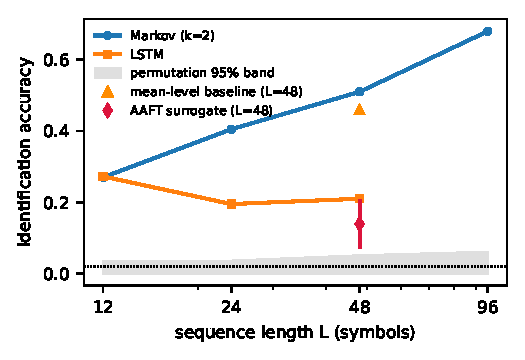
\includegraphics[width=\columnwidth]{fig1_accuracy_vs_L.pdf}
\caption{Test-A accuracy vs.\ sequence length ($N{=}50$). Markov exceeds the
permutation band at all $L$; the LSTM trails; the AAFT surrogate and mean-level
points quantify the two controls.}
\label{fig:accL}
\end{figure}

\begin{figure}[t]
\centering
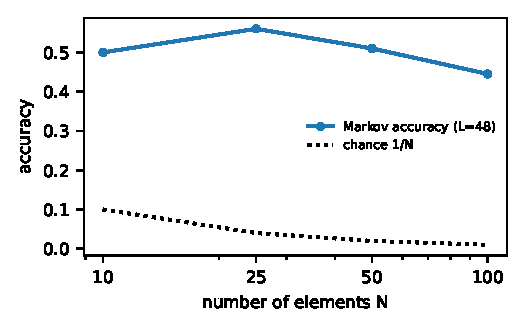
\includegraphics[width=0.86\columnwidth]{fig2_accuracy_vs_N.pdf}
\caption{Test-A accuracy vs.\ element count $N$ ($L{=}48$) against the $1/N$
chance line.}
\label{fig:accN}
\end{figure}

\begin{figure}[t]
\centering
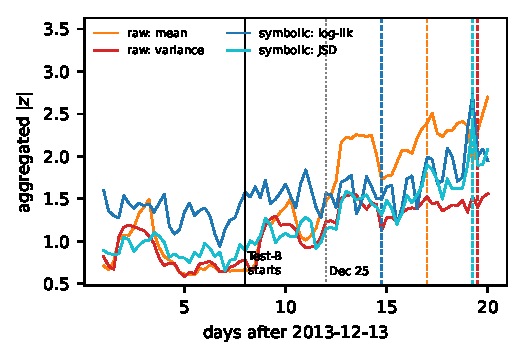
\includegraphics[width=\columnwidth]{fig3_drift.pdf}
\caption{H3: aggregated deviation of symbolic and raw signals through Test-B.
Dashed verticals mark CUSUM alarms; the symbolic log-likelihood alarms
earliest.}
\label{fig:drift}
\end{figure}

\section{Discussion}
\textbf{Operational upside.} A shallow, cheap symbolic model passively
identifies the source cell of aggregated telemetry from short windows, and its
grammar drifts $\sim\!2$ days before mean/variance during a load regime change.
This supports passive element identification and early configuration-/regime-drift
detection from data an operator already collects, without per-packet inspection.

\textbf{Security/privacy downside.} The same mechanism is an
infrastructure-fingerprinting vector: because identification works on
coarse, aggregated, z-normalized activity, an observer who sees only volume
envelopes---plausibly behind encryption or aggregation---can still
distinguish and track individual elements. Normalization does not protect the
element: it merely shifts the discriminative signal from volume to grammar,
and both remain exploitable. This argues for treating aggregate telemetry
envelopes as identifying data.

\textbf{Substrate independence.} Our only quantitative cross-substrate claim is
the H2 comparison, and it is \emph{negative}: the Milano threshold does not
match the prior quantum/EEG relation (Table~\ref{tab:h2}). We make no claim of a
universal law.

\section{Limitations}
Results are from one dataset, one channel, and one city; generality is
untested. The strongest limitation is the volume confound: a trivial mean-level
classifier rivals or beats the grammatical one at small $N$, so ``fingerprint''
must be read as volume-plus-grammar, with grammar isolated only after
normalization. The AAFT surrogate leaves a residual $7\times$-chance marginal
component, so the grammatical share, though dominant, is not total. $N^\ast$ is
left-censored below our shortest window, so H2 places only an upper bound; a
finer short-$L$ grid could localize it but was not pre-registered and was not
added. The prior scaling relation could not be verified in the literature and
is treated as a proposal. The LSTM was deliberately small and lightly tuned;
a larger model with more per-element data might close the gap to the shallow
baseline, though it is not needed for the central claim.

\section{Conclusion}
Network elements do have a grammatical fingerprint: a shallow Markov model over
SAX symbols identifies the source cell far above chance ($0.51$ vs.\ $0.02$ at
$N{=}50$, $p<0.001$), the signal is largely temporal (surrogate accuracy
$0.139$), it is detectable from very short sequences ($N^\ast<12$ symbols), and
it drifts a median $54$\,h before first-order metrics. The fingerprint is real
and volume-independent, but coexists with an equally real volume fingerprint,
and its data threshold is inconsistent with the authors' prior scaling
proposal. A sequence model was unnecessary. The honest summary is a supported
central claim wrapped in two negative findings---a competing confound and a
failed scaling law---reported with equal weight.

\section*{Disclosure Statement}
\textbf{Model and framework.} All technical content---design, code, analysis,
figures, and text---was produced by an autonomous agent (Anthropic Claude,
Fable~5) driving the Claude Code / Agent SDK harness. \textbf{Human role.} The
human supplied the starting prompt and made procedural decisions only:
interventions were (1) initial prompt; (2) one \emph{reject} (plan incomplete:
H2 mapping and H1/H3 confound), which the agent fixed; (3) one \emph{accept}
with a clarifying condition on surrogate generation; (4) one procedural
authorization of the email used for the dataset's mandatory download guestbook.
The human wrote no technical content, numbers, citations, or wording.
\textbf{Pre-registration.} The complete starting prompt, the pre-registered
plan, the hyperparameter-freeze commit preceding the single test evaluation,
the full commit history, seeds, and the interaction transcript are in the
public repository. \textbf{Reproducibility.} \texttt{python reproduce.py
{-}{-}email <addr>} regenerates every table and figure (global seed 42).
\textbf{Repository.} \url{https://github.com/<to-be-inserted-on-submission>}.

\bibliographystyle{IEEEtran}
\bibliography{refs}

\end{document}
